% 02.06.2016 12:00 CET last changed by a.holzinger
% General Template for LNCS and LNAI contributions based on llncs, adapted by ah
% Many thanks to the TRS team
% In case of using eps compile via 1) TeXify and then proceed with 2) dvi2pdf
%
\documentclass{llncs}
\usepackage{float}

\usepackage[dvips]{graphicx}
\usepackage[ruled,vlined]{algorithm2e}
\usepackage{amsfonts}
\usepackage{amssymb}
\usepackage{amsmath}
\usepackage{mathtools}

\providecommand{\abs}[1]{\lvert#1\rvert}
\providecommand{\norm}[1]{\lVert#1\rVert}

\usepackage{calc}
\usepackage{subfigure}

\usepackage{color}
\usepackage{soul}
\usepackage{comment}

\newtheorem{prop}{Property}

\newenvironment{Bitemize}{\renewcommand\labelitemi{\textbullet}\begin{itemize}}{\end{itemize}}

\begin{document}

\title{Interactive Anonymization\\
for Privacy aware Machine Learning}

\author{Bernd Malle\inst{1}\inst{2}, Peter Kieseberg\inst{1}\inst{2}, Andreas Holzinger\inst{1}}

\institute{Holzinger Group HCI-KDD \\
Institute for Medical Informatics, Statistics \& Documentation\\
            Medical University Graz, Austria\\
            \texttt{b.malle@hci-kdd.org}
\and
SBA Research gGmbH, Favoritenstraße 16, 1040 Wien \\
			\texttt{PKieseberg@sba-research.org}
}
	
\maketitle

% ==================================
%				ABSTRACT
% ==================================
\begin{abstract}




\medskip

\textbf{Keywords}: Machine Learning, Privacy aware ML, interactive ML, Knowledge Bases, Anonymization, k-Anonymity, SaNGreeA, Information Loss, Weight Vectors


\end{abstract}

\renewcommand{\thesubfigure}{\thefigure.\arabic{subfigure}}
\makeatletter
\renewcommand{\p@subfigure}{}
\renewcommand{\@thesubfigure}{\thesubfigure:\hskip\subfiglabelskip}
\makeatother


% ==================================
%			INTRODCUTION
% ==================================
\section{Introduction and Motivation}
\label{sect:intro_moti}


% ==================================
%			    PAML
% ==================================
\section{Privacy aware Machine Learning}
\label{sect:paml}


% ==================================
%			  PRIVACY
% ==================================
\section{Methods of providing privacy}
\label{sect:methods_privacy}

\subsection{Perturbation}
\label{ssect:perturbation}

\subsection{$\epsilon$  differential privacy}
\label{ssect:eps_priv}

\subsection{k-anonymity (and beyond)}
\label{ssect:k_anon}

Figure~\ref{fig:anon_categories} illustrates the original tabular concept of anonymization: Given an input table with several columns, we will in all probability encounter three different categories of data:


\begin{figure}[!t]
	\begin{center}
		%		\includegraphics[width=\textwidth]{figures/anonym/gen_hierarchy}
		\caption{Example of a typical generalization hierarchy}
		\label{fig:gen_hierarchy}
		\small
		taken from \cite{aggarwal2005approximation}
	\end{center}
\end{figure}


\begin{itemize}
	\item \textbf{Personal identifiers} are data items which directly identify a person without having to cross-reference or further analyze them. Examples are first and last names, but even more so an (email) address or social security number (SSN). As personal identifiers are dangerous and cannot be generalized (see Figure~\ref{fig:gen_hierarchy}) in a meaningful way (e.g. one could generalize an email address by only retaining the mail provider fragment, but the result would not yield much usable information), this category of data is usually removed. The table shows this column in a red background color.
	\item \textbf{Sensitive data,} also called 'payload', which is the kind of data we want to convey for statistics or research purposes. Examples for this category would be disease classification, drug intake or personal income level. This data shall be preserved in the anonymized dataset and can therefore not be deleted or generalized. The table shows this column in a green background color.
	\item \textbf{Quasi identifiers (QI's)}, colored in the table with an orange background, are data that in themselves do not directly reveal the identity of a person, but might be used in aggregate to reconstruct it. For instance, \cite{sweeney2002k} mentioned that 87\% of U.S. citizens in 2002 had reported characteristics that made them vulnerable to identification based on just the 3 attributes \textit{zip code}, \textit{gender} and \textit{date of birth}. But although this data can be harmful in that respect, it might also hold vital information for the purpose of research (e.g. zip code could be of high value in a study on disease spread). The the actual point of all anonymization efforts is therefore to generalize this kind of information, which means to lower its level of granularity. As an example, one could generalize the ZIP codes 41074, 41075 and 41099 to an umbrella version 410**, as shown in Figure~\ref{fig:anonymized_clusters}.
\end{itemize}



% ==================================
%				iML
% ==================================
\section{interactive Machine Learning}
\label{sect:iML}



% ==================================
%			EXPERIMENTS
% ==================================
\section{Experiments}
\label{sect:experiments}

The following sections will describe our series of experiments in detail, encompassing the data source selected, the algorithm used as well as a description of the overall process employed to obtain our results.


\subsection{Data} 
\label{ssect:data}

As input data we chose the adults dataset from the UCI Machine Learning repository which was generated from US census data of 1994 and contains approximately 32,000 entries; from those 30,162 were selected after preprocessing. Of the attributes (data columns) provided only one was deleted because it was also represented by a column containing its numerical mapping (education $=>$ education\_num). Figure~\ref{fig:adult_original_distribution} shows the attribute value distribution of the original input dataset with the exception of the sample weights.


\begin{figure}[!t]
	\begin{center}
    \hspace*{-0.8cm}
%		\includegraphics[width=1.1\textwidth]{figures/experiment/dist_initial_small}
		\caption{Initial distribution of six selected data columns of the adult dataset.}
		\label{fig:adult_original_distribution}
	\end{center}
\end{figure}

As one can see, there are several attributes with one value clearly dominating the others; \textit{native-country} being the most prominent example with the entry for the United States dwarfing all other countries (which comes as no surprise given the data origin). As anonymization generalizes different countries together if necessary, it was interesting for the author to see how these distributions would change under a relatively large k-factor. Figure~\ref{fig:adult_anonymized_distribution} shows the same attribute distribution with its values anonymized by a factor of $k=19$. Although the dominance of the United states was successfully "broken" by this method, in several instances the \textit{generalized-to-all}-value (*) now skews the data set even more. Apart from the expected generalization information loss this is another reason why one would assume worse results from a machine learning classifier applied to an anonymized dataset.

\begin{figure}[!t]
	\begin{center}
    	\hspace*{-0.8cm}
%		\includegraphics[width=1.1\textwidth]{figures/experiment/dist_anonym_small}
		\caption{Anonymized distribution of six selected data columns of the adult dataset, anonymization factor of k=19, equal weight for each attribute.}
		\label{fig:adult_anonymized_distribution}
	\end{center}
\end{figure}



\subsection{Algorithm}
\label{ssect:algorithm}

SaNGreeA stands for \textit{Social network greedy clustering} and was introduced by \cite{campan2009data}. In addition to 'clustering' nodes of a graph according to the minimum general information loss (GIL) incurred as described in Section~\ref{ssect:tab_anonym}, this algorithm also considers the structural information loss (SIL) incurred in assigning a node to a certain cluster. The SIL quantifies the probability of error when trying to reconstruct the structure of the initial graph from its anonymized version.

\begin{equation*}
\begin{split}
\text{GIL}(cl) = \abs{cl} \cdot (\sum_{j=1}^{s} \frac{size(gen(cl)[N_j])}{size(min_{x \epsilon N} (X[N_j]), max_{x \epsilon N} (X[N_j]))} \\
+ \sum_{j=1}^{t} \frac{height(\Lambda(gen(cl)[C_j]))}{height(H_{C_j})})
\end{split}
\end{equation*}


where:\\
- $\abs{cl}$ denotes the cluster cl's cardinality; \\
- $size([i1,i2])$ is the size of the interval $[i1,i2]$, i.e., $(i2-i1)$; \\
- $\Lambda(w), w \epsilon H_{C_j}$ is the sub-hierarchy of $H_{C_j}$ rooted in $w$; \\
- $height(H_{C_j})$ denotes the height of the tree hierarchy $H_{C_j}$; \\


The total generalization information loss is then given by:
\begin{equation*}
\text{GIL}(G,S) = \sum_{j=1}^{v} \text{GIL}(cl_j)
\end{equation*}
And the normalized generalization information loss by:
\begin{equation*}
\text{NGIL}(G,S) = \frac{\text{GIL}(G,S)}{n \cdot (s+t)}
\end{equation*}


\subsection{Process}
\label{ssect:process}

To examine the impact of perturbation and anonymization of datasets on the quality of a classification result, we designed the following processing pipeline:


\begin{enumerate}
	\item Taking the original (preprocessed) dataset as input, we transformed its attributes to boolean values, so instead of \textit{native-country $->$ United-States} we considered \textit{United-States $->$ yes / no}.
	% \item A correlation matrix of the resulting binary feature set was computed to get a better feeling for the data (see Figure~\ref{fig:adult_correlation_big}).
	\item We then ran 4 different classifiers on it and computed precision, recall as well as F1 score. The four classifiers used were \textit{gradient boosting}, \textit{random forest}, \textit{logistic regression} and \textit{linear SVC}.
	\item From the obtained results we extracted the 3 attribute values most contributing to a "positive" ($>$50k) result as well as the top 3 attribute values indicating a "negative" ($<=$50k) prediction as depicted in Figure~\ref{fig:adult_important_columns}
	\item For each of these 6 attribute values, we subsequently deleted a specific percentage of data rows containing that value from the original dataset, resulting in 30 reduced datasets. The 5 percentages used were $0.2$, $0.4$, $0.6$, $0.8$ as well as $1.0$.
	\item To each of those datasets we re-applied the four chosen classifiers successively and recorded the respective impact on the quality of the classification result. The results can be seen in Figure~\ref{fig:adult_results_perturbation_top} and Figure~\ref{fig:adult_results_perturbation_bottom}.
	\item In order to measure the effects of k-anonymization on classifier performance, we used the SaNGreeA's GIL component described in the following section to generate datasets with a k-factor of $k=3$, $k=7$, $k=11$, $k=15$ as well as $k=19$. Furthermore, we used each of these settings with 3 different weight vectors: 1) equal weights for all attributes, 2) age information preferred ($\omega(age)=0.88$, $\omega(other\_attributes)=0.01$) and 3) race information preferred ($\omega(race)=0.88$, $\omega(other\_attributes)=0.01$). We then re-executed all classifiers on the resulting 15 datasets and recorded the respective results, which can be seen in Figure~\ref{fig:adult_results_anonymization}.
\end{enumerate}


\begin{figure}[!t]
	\begin{center}
		\vspace{-1.0cm}
    	\hspace*{-0.8cm}
		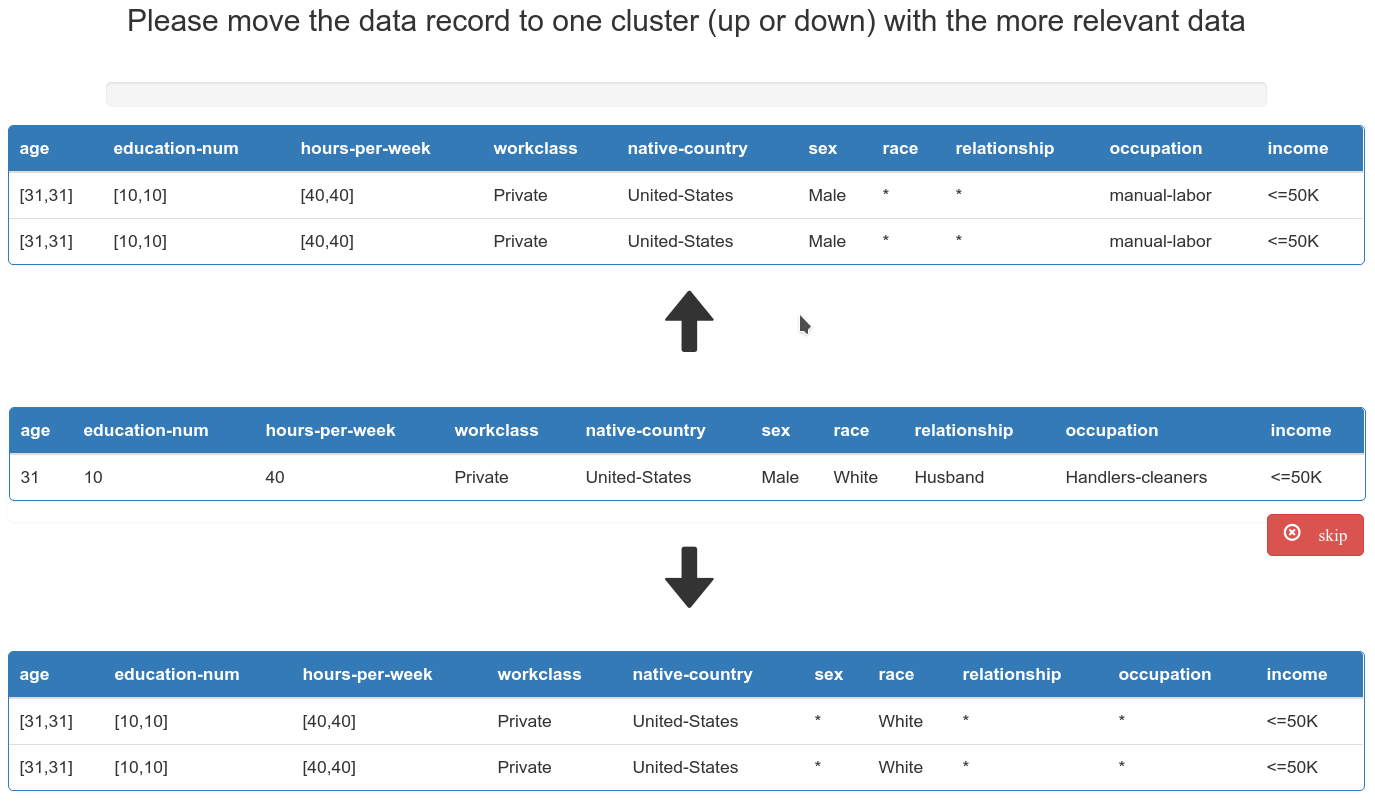
\includegraphics[width=1.0\textwidth]{figures/iml_anon_screen1}
		
		\vspace{1.0cm}
		\hspace*{-0.8cm}
		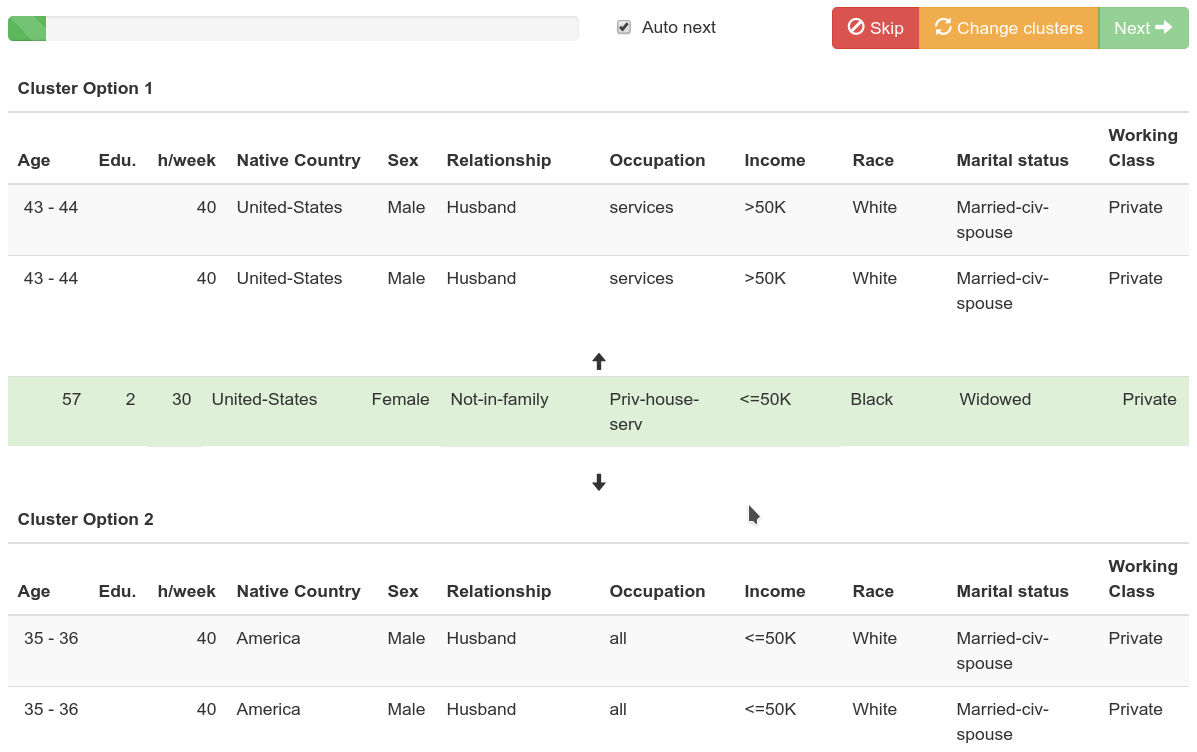
\includegraphics[width=1.0\textwidth]{figures/iml_anon_screen2}
		\caption{Two implementations of the iML interface design...}
		\label{fig:adult_important_columns}
	\end{center}
\end{figure}


% ==================================
%		RESULTS & DISCUSSION
% ==================================
\section{Results \& Discussion}
\label{sect:results}

\begin{figure}[!h]
	\begin{center}
		\vspace{-1.0cm}
		\hspace*{-0.8cm}
		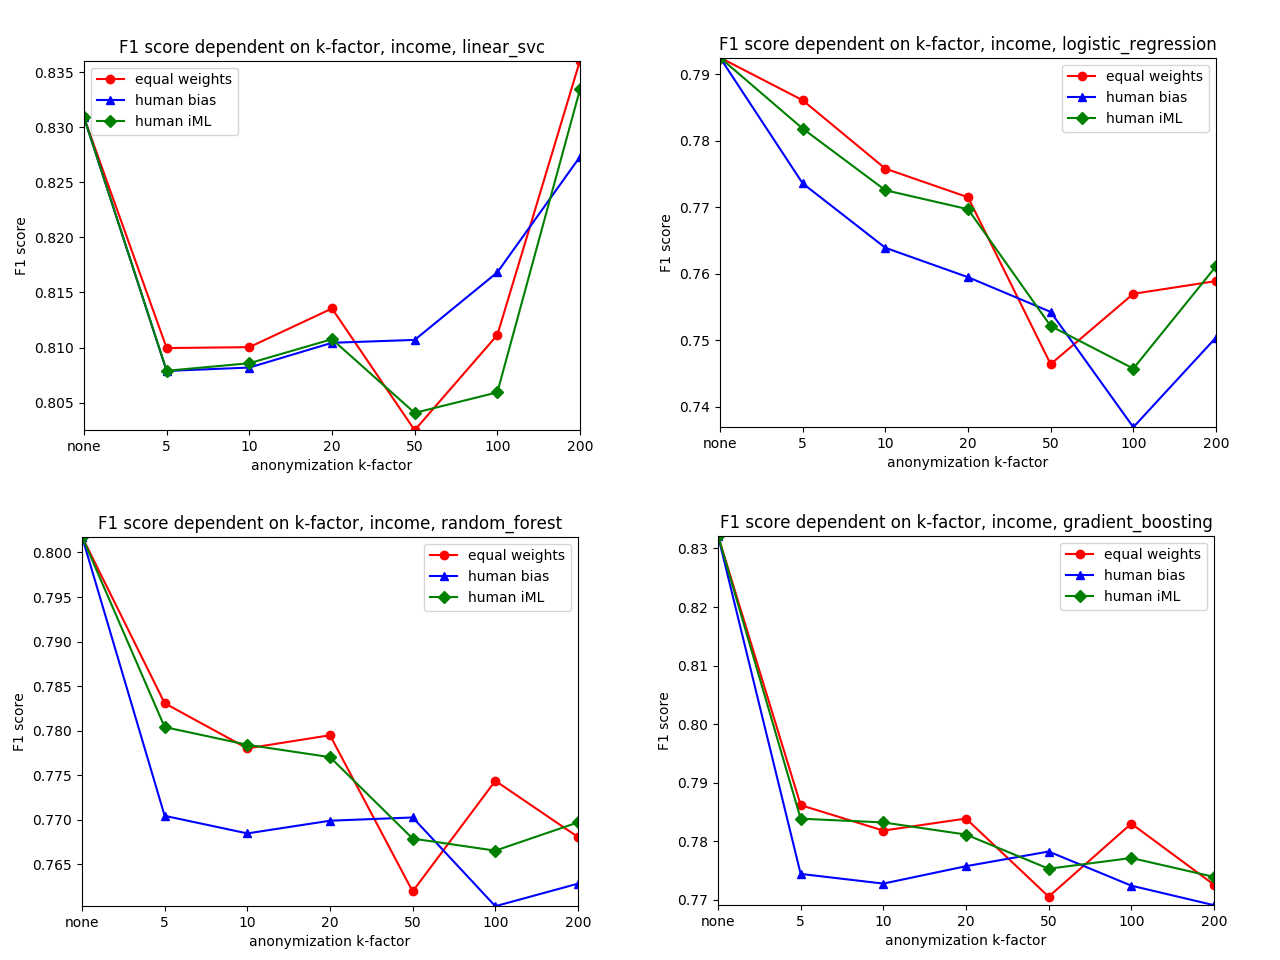
\includegraphics[width=1.0\textwidth]{figures/income.png}
		\caption{Results on...}
		\label{fig:results_income}
	\end{center}
\end{figure}

\begin{figure}[!h]
	\begin{center}
		\vspace{-1.0cm}
		\hspace*{-0.8cm}
		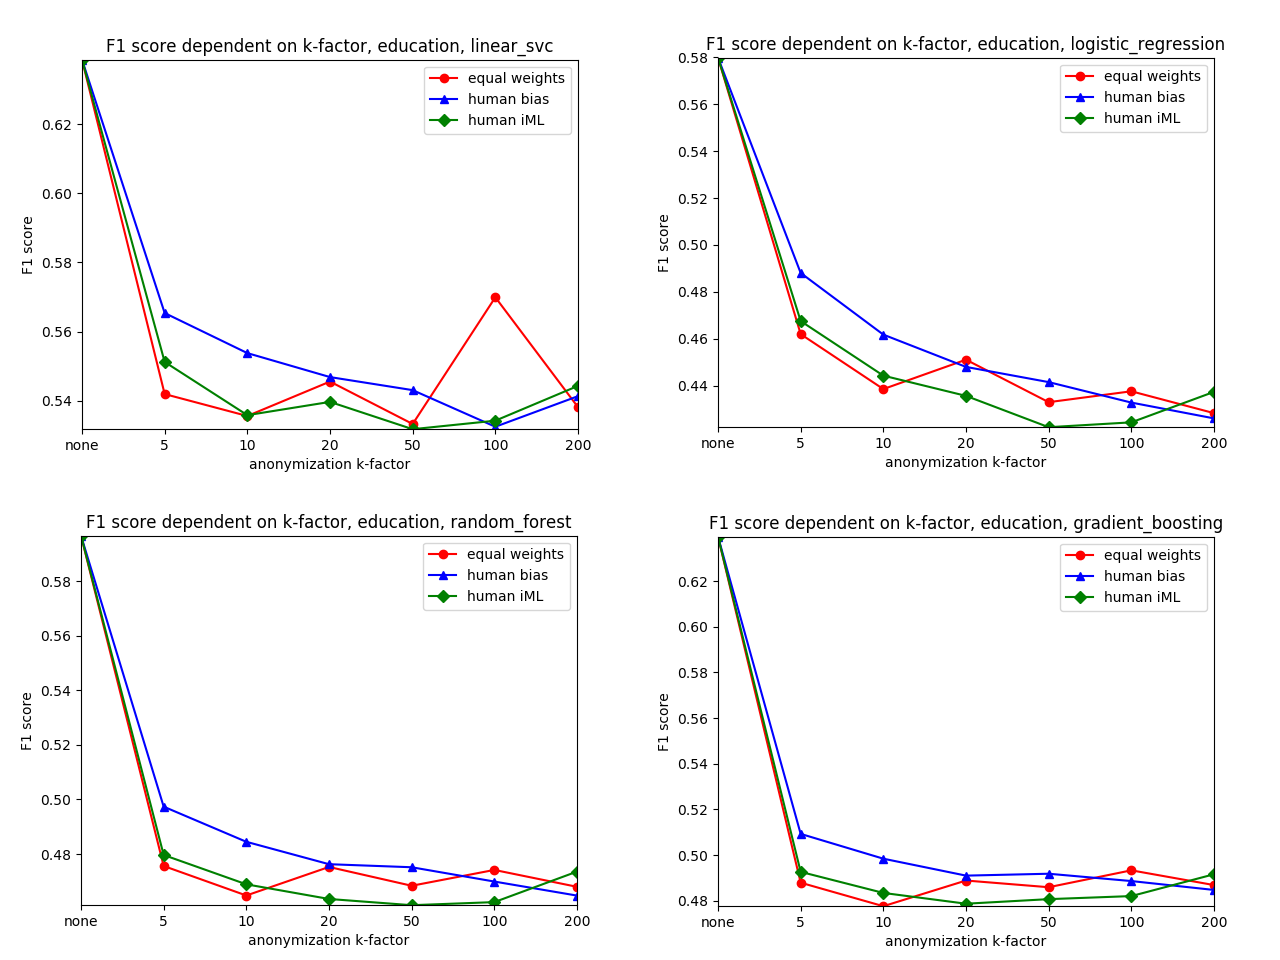
\includegraphics[width=1.0\textwidth]{figures/education_num.png}
		\caption{Results on...}
		\label{fig:results_income}
	\end{center}
\end{figure}

\begin{figure}[!h]
	\begin{center}
		\vspace{-1.0cm}
		\hspace*{-0.8cm}
		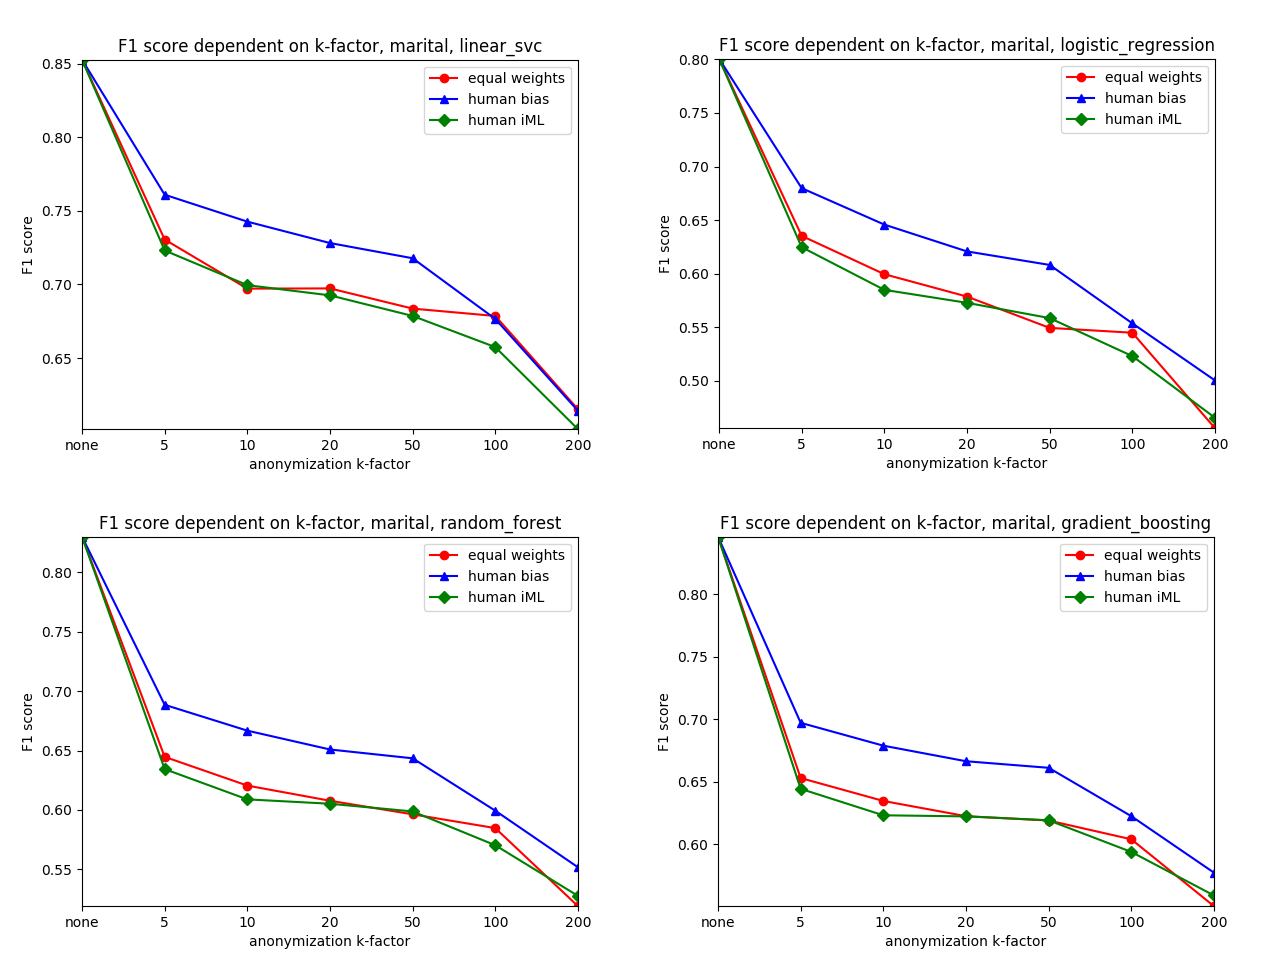
\includegraphics[width=1.0\textwidth]{figures/marital_status.png}
		\caption{Results on...}
		\label{fig:results_income}
	\end{center}
\end{figure}



% ==================================
%		PROBLEMS & CHALLENGES
% ==================================
\section{Open problems \& future challenges}
\label{sect:op_fc}

\begin{itemize}
	\item \textbf{Explain the unexpected behavior} for...
\end{itemize}


% ==================================
%			CONCLUSION
% ==================================
\section{Conclusion}
\label{sect:conclusion}


\newpage

\bibliographystyle{plain}
\bibliography{references}

\end{document}

